\section{BranchConnect: The Game}
\label{sec:game}
The online game is accessible by laptops and mobile touch devices, and many users can play at the same time.
The objective of the game is to collect valid layouts of branches which are fabricatable with 3 axis CNC milling machines.
By analyzing the connectivity of branches and target points, the game informs the feasibility of a given layout.
Similar to our game, the work \textit{guidance system during furniture design} inspected connectivity, durability, and stability \cite{umetani2012guided}.
Unlike their work, our game puts emphasis on \textit{fabricatability}, as well as \textit{geometric connectivity}, and does not calculate structural performance of each joint.
Instead we use simple geometric analysis to compute validity.
We also assume that every fabricated joint works as a rigid joint, thus single connection is counted as stable to hold a pair of branches.

The overall user experience is as follows.
In the selection interface (Figure \ref{fig:game_interface} left), each frame comes with a set of predefined target points to be connected.
The distribution of these target points is predefined by the system, and end users can not modify them.
After a user selects a target frame and a set of branches on a plate, the user is guided to the game interface (Figure \ref{fig:game_interface} right), consisting of the frame with the target points, and the set of available branches at the bottom.
The user picks a branch from the available set on the bottom, and drag\&drop it to the inside of the target frame.
By selecting and dragging these dropped branches, the user searches a good 2D pose through basic direct geometric manipulations such as move, rotate, and horizontal flip (or mirror).
While the manipulation, the user receives simple feedback with colors and score.
Within the limited number of available branches, the user needs to bridge all the target points by connecting all the dropped branches in one group.
The game is completed when all the target points are connected.
To achieve higher score, the user can keep modifying the design, and save it to the database.

\begin{figure}[ht]
  \begin{center}
    
\includegraphics[width = 0.4\paperwidth]{images/interface/game_interface.png}
    \caption{Left: the selection interface for target frames (top) and branch panels (bottom). Right: the start interface of the game.}
    \label{fig:game_interface}
  \end{center}
\end{figure}
%
\subsection{The Game System}
There are many physics simulation libraries for game, however, our game needs to detect intersected branch pairs, thus collision detection with physics engines is overkill for our browser game.
%Our game is running on browsers with rich
Also, branches have free-form concave shapes, thus further geometric preparation such as convex decomposition is necessary for using these libraries.
For fast and robust intersection detection, our game extensively uses down-sampled skeletons of branches.

Hubbard and Philip developed collision detection by representing an object with hierarchical 3D spheres aligned on a skeleton \cite{Hubbard:1996:APS:231731.231732}.
Our game takes similar approach but limited in 2D.
Instead, we put more emphasis on searching fabricatable joints.
In the game, down-sampled skeletons are used to find the pair of closest skeleton points between two branches.
While a branch is selected, the system searches the closest skeleton point of the selected branch with other skeletons of available branches.
If the distance of a pair of the closest skeleton points is smaller than a threshold, the pair is intersected.
More precise joint calculation with high-resolution contours is further described in Section \ref{sec:fabrication}.


Here, we introduce two important entities in the game: joint and group.
A joint is created when an intersecting pair is detected, and the pair forms a group.
The group is used for evaluating connections between target points.
The conditions of joint and group are indicated with simple color-code.
Once the user finishes geometric manipulation, score is updated with weighted sum of score parameters.
Together with the color-code, the score update guides the user to form a feasible design.



\subsubsection{Joint Condition}
\label{sec:joint}
Joint is the essential entity not only in the game but also in the fabrication process of customized lapped joints.
Importantly, each pair of branches must have one flipped branch for fabrication constraint (Section \ref{sec:fabrication}).
Together with this constraint, we set several valid and invalid contraints illustrated in Figure~\ref{fig:joint_condition}.
Our joint takes only crossed pair because they are structurally stable, relatively simple to fabricate, and creates diverse designs (Figure~\ref{fig:joint_condition}.1).
Due to fabrication process with CNC milling, we do not take conditions such as terminal connection, joint at metal fixture, and T-shaped connection (Figure~\ref{fig:joint_condition}.3, \ref{fig:joint_condition}.4, and \ref{fig:joint_condition}.5 respectively) .
A valid joint's angle stays within a fixed range (Figure~\ref{fig:joint_condition}.1 and 2).
Valid and invalid joints are displayed with green and red respectively.

\begin{figure}[ht]
	\begin{center}
		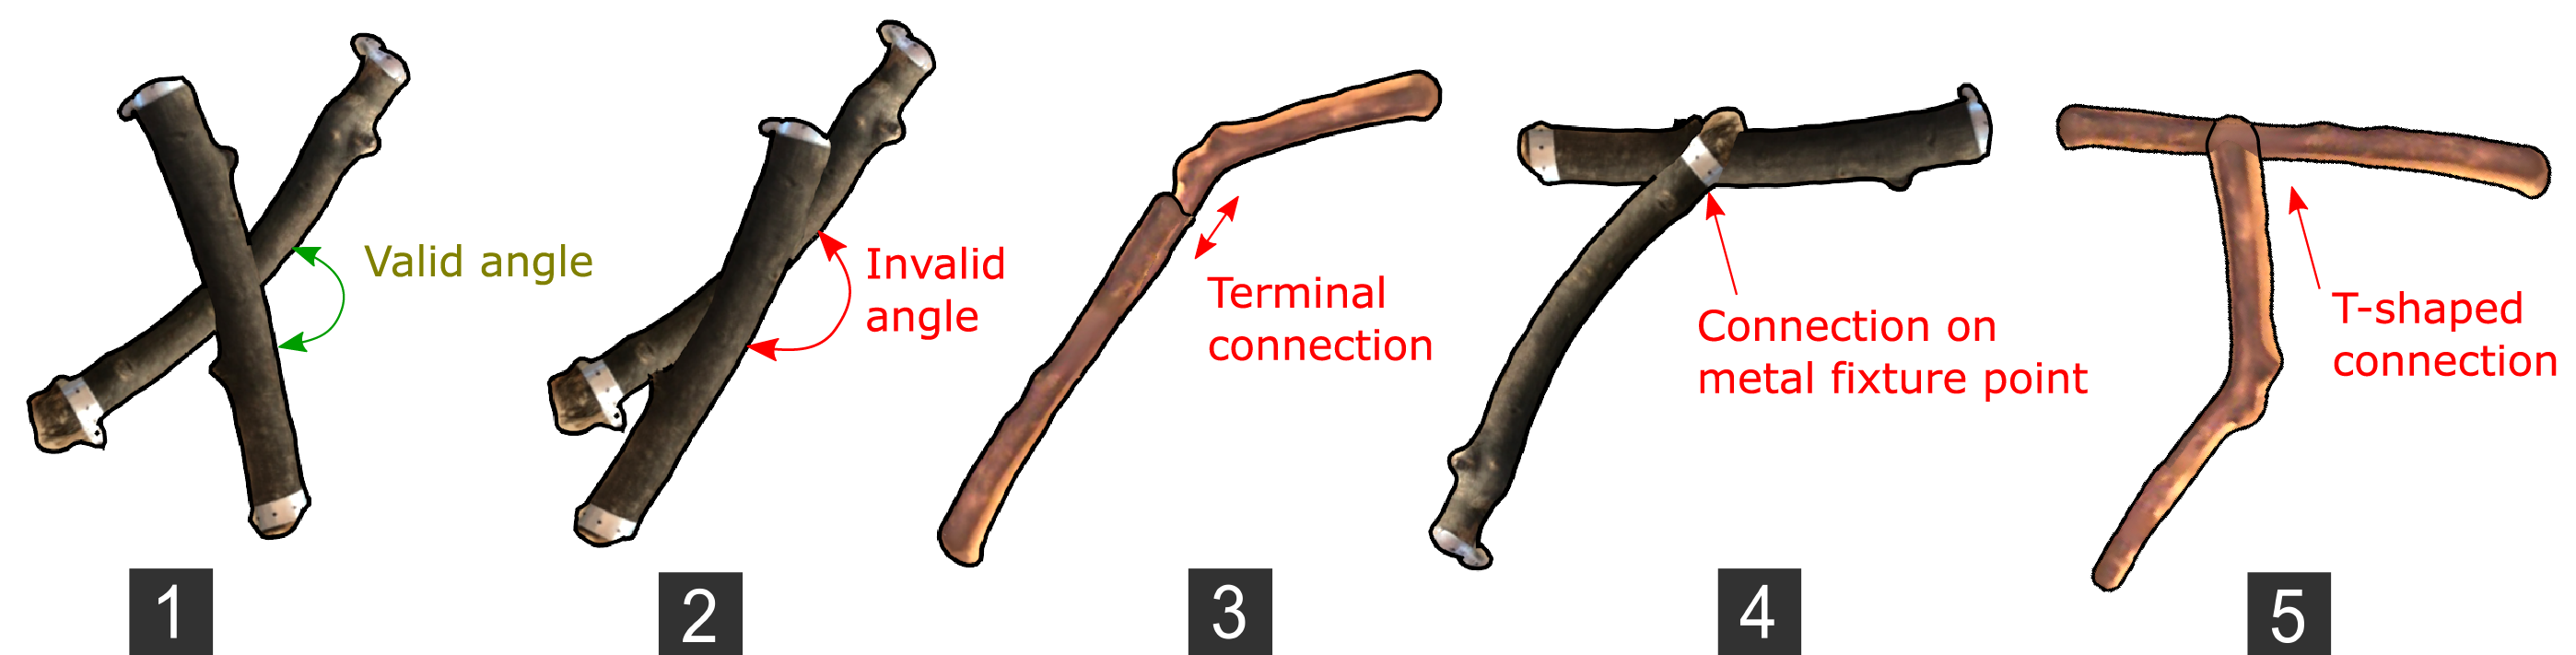
\includegraphics[width = 0.4\paperwidth]{images/system/joint_conditions_3.png}
		\caption{Joint conditions. 1. valid joint. 2. invalid for violating the angle. 3. invalid terminal connection. 4. invalid for connecting on a metal fixture point. 5. invalid for T-shaped connection.}
		\label{fig:joint_condition}
	\end{center}
\end{figure}




To describe the joint update process, let each branch $b_i$ be a member of a set of the branches $\mathcal{B}$ dropped inside of the target frame by a user.
The user freely selects $\mathcal{B} \in \mathcal{B_\text{plate}}$, where $\mathcal{B_\text{plate}}$ is the branches fixed on a selected plate.
Note that we accept one joint with a pair of branches, but a branch can have multiple joints with other branches.
The process starts from the selected branch $b_i$ and updates joint conditions of the selected branch with paired branches.
When an intersected pair is detected, it stores $j$-th joint $j_{i, j}$ in $b_i$ as joint conditions.
After evaluation, as in Figure \ref{fig:joint_condition},  we have joints labeled as valid or invalid.
When a branch $b_i$ is connected to one of target points $t_j \in \mathcal{T}$, the target point $t_{i, j}$ is stored in $b_i$.
Note that we also take one target point per branch.
The branch connected to the target point is trimmed at the target point.
The trimmed length $l_{\text{trim}, i}$ is stored in $b_i$ and use as a penalty for score calculation.
In this way, the user tries to position the branch as inside of the frame as possible.
This process is iteratively executed while a user is positioning a branch while dragging.


%\begin{figure}[h]
%	\begin{center}
%		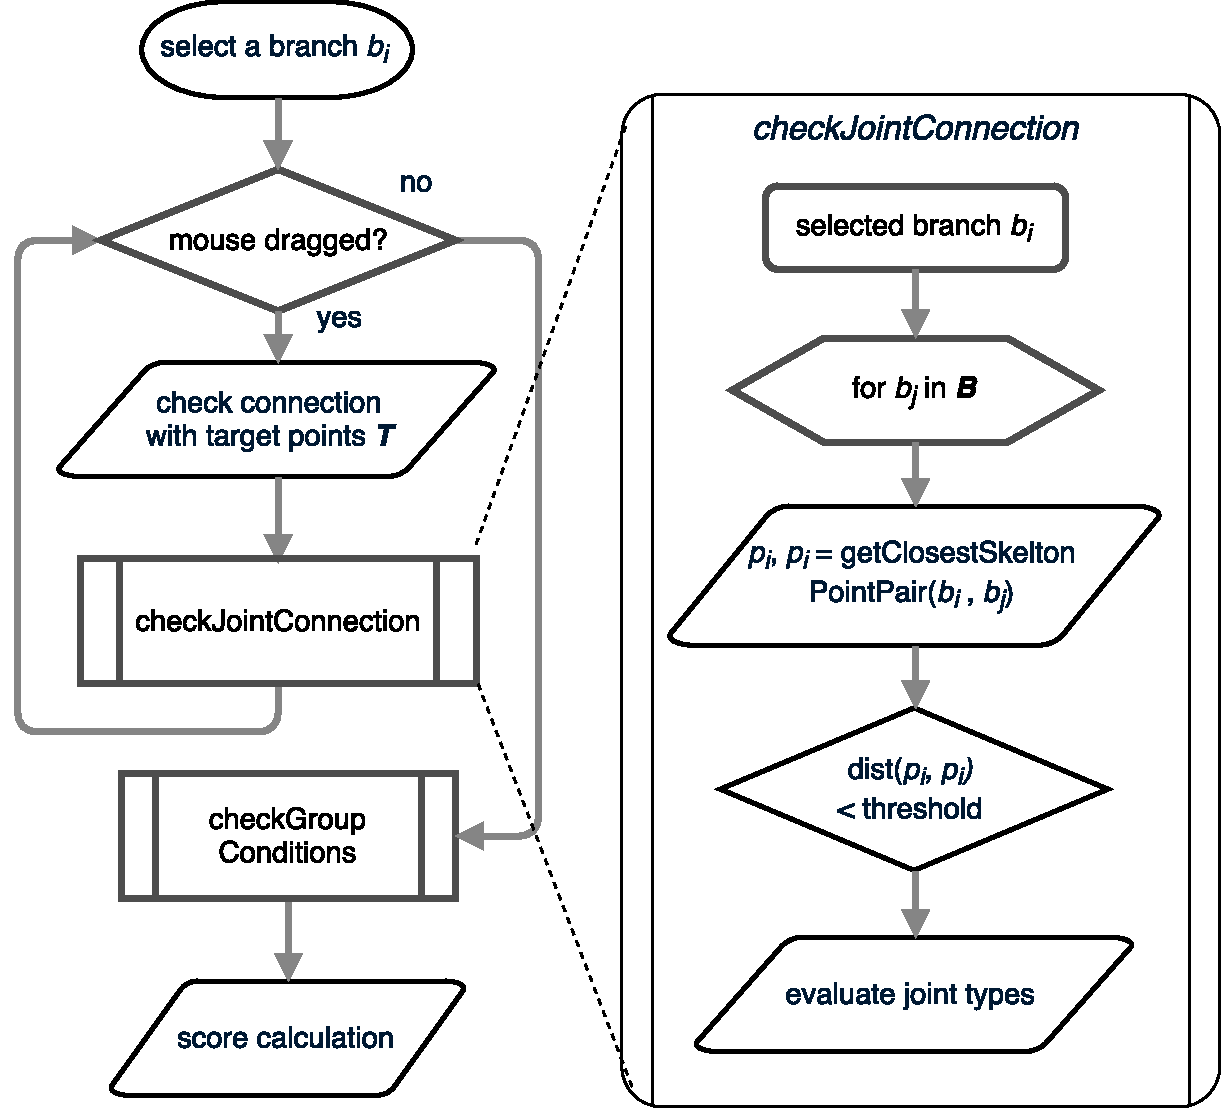
\includegraphics[width = 0.35\paperwidth]{images/system/closestPointAlgorithm.pdf}
%		\caption{Left: an overview of the game system with 1. joint update 2. group update and 3. score calculation. This process is iteratively executed while a user is exploring layout by dragging a branch. The joint update process is further illustrated in the right, and group condition update is described in Algorithm \ref{al:connection}. }
%		\label{fig:system_flowchart}
%	\end{center}
%\end{figure}

% well as the paired branch $b_{\text{paired},j} \in \mathcal{P}_{\text{paired},i}}$.



\subsubsection{Group Condition}

After a user finishes positioning a branch, the system groups a set of connected branches together.
% For detail procedure of this process, please refer Appendix 1.
Firstly it updates groups, and then detects invalid group conditions, as well as connections to target points.
If a branch is connected to a target point, colors of the branch and its belonging group are updated, informing users about the validity of their layouts.
When a group bridges a pair of target points, a special score is added and displayed with an animation.

After updating the group, the process evaluates the connections with target points.
Denoting a group and a set of groups as $g_k$ and $\mathcal{G}$ respectively, we check each branch $b_i \in g_k \in \mathcal{G}$ whether it has a connection with a target point or not. If it has, the target point is stored in the group $g_k$.
If multiple groups with target points for each exist, the entire structure is feasible, however, these groups should be connected together (Figure \ref{fig:group} middle).
If the group does not have any target point, the group is labeled as \textit{Islanded}, which is structurally infeasible thus counted as a penalty in the cost calculation (Figure \ref{fig:group} right).
If the group has multiple target points, these target points are bridged.
The game completes when the number of $\mathcal{G}$ is one, and all the target points are connected with the group, which does not have branches with invalid joints.

\begin{figure}[ht]
  \begin{center}
    
\includegraphics[width = 0.4\paperwidth]{images/interface/groups.jpg}
    \caption{Left: valid group with two target points connected. Middle: valid but three groups. Right: invalid due to the \textit{Islanded} situation. }
    \label{fig:group}
  \end{center}
\end{figure}

\subsubsection{Score Calculation}
We calculate the score with weighted sum of following entities: the numbers of valid and invalid joints on each branch as $N$($\mathcal{J}_{\text{valid},i}$) and  $N$($\mathcal{J}_{\text{invalid},i}$) respectively, the number of groups as $N(\mathcal{G} )$, the number of islanded groups as $N(g_{\text{islanded}})$, the number of bridged target points as $N(t_{\text{bridged}, i})$.
The trimmed length $l_{\text{trim}, i}$ in each $b_i \in \mathcal{B}$.
The score is weighted sum of these joint and group conditions, denoted in Equation (\ref{eq:score}).
The weights $w_1 \dotso  w_5$ are non-negative weight coefficients pre-adjusted in advance by the authors.


\begin{equation}
 \begin{aligned}
 Score =  &\; w_1\;  \sum_{1}^{N(\mathcal{B})} N(\mathcal{J}_{\text{valid},i})\; +  \;w_2\; \sum_{1}^{N(\mathcal{B})} N(\mathcal{J}_{\text{invalid},i})\\
		+ &\; w_3\;  N(g_{\text{islanded}} \in \mathcal{G} )\;				 	 \;+  \;w_4\;  N(t_{\text{bridged}, i}) \; +  \;w_5\; \sum_{1}^{N(\mathcal{B})} l_{\text{trim}, i}
 \\
   \textrm{s.t.} & \; w_j  \in \mathbb{R} \; \wedge \;   \forall j \in 1, \dotsc , 5
 \end{aligned}
 \label{eq:score}
\end{equation}
